Pasek umieszczony po lewej stronie ekranu nosi nazwę Launchera (ang: \textcolor{ubuntu_orange}{Wyzwalacz}). Launcher umożliwia przechowywanie skrótów do ulubionych i najczęściej używanych aplikacji, dostęp do uruchomionych programów, zamontowanych urządzeń (pamięć USB/SD, zewnętrzne dyski twarde, CD/DVD) oraz kosza. Uruchomiona aplikacja na czas swojej pracy umieszcza w Launcherze swoją ikonę.

\subsubsection{Uruchamianie programów z Launchera}
\begin{wrapfigure}{l}{0.1\textwidth}
	\vspace{-10pt}
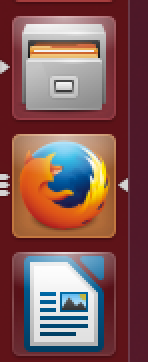
\includegraphics[width=\linewidth]{images/unity_launcher_programy.png}
\end{wrapfigure}

Aby uruchomić program bezpośrednio z Launchera, wystarczy pojedyncze kliknięcie ikony wybranego programu lewym przyciskiem myszy. Uruchomione programy mają podświetlone ikony oraz niewielki trójkącik po lewej stronie. Aby uruchomić kolejną kopię programu, kliknij jego ikonę lewym przyciskiem myszy, trzymając wciśnięty klawisz \keys{Shift}.

\noindent Liczba trójkątów po lewej stronie programu oznacza ilość otwartych kopii danego programu. Jak łatwo się domyślić, gdy ikona nie ma żadnego trójkącika, to program jest wyłączony. Program, którego aktualnie używamy (aktywne okno), jest oznaczony trójkącikiem po prawej stronie ikony.

\noindent Na rysunku obok widzimy ikonę programu Pliki (menadżer plików Nautilus), który jest uruchomiony jeden raz. Tło ikony jest podświetlone.\\
Ikona przeglądarki internetowej Firefox ma trzy trójkąty po lewej. Oznacza to, że została uruchomiona w trzech osobnych instancjach. Jedna z kopii Firefoksa jest akurat w użyciu, co sygnalizuje trójkącik po prawej. Tło ikony jest podświetlone.\\
Trzecia ikona na rynku (skrót do procesora tekstu LibreOffice Writer) jest nieaktywna. Ten program nie jest aktualnie uruchomiony.

\subsubsection{Zarządzanie otwartymi oknami}
Kliknięcie ikony uruchomionego programu lewym przyciskiem myszy przenosi do otwartego okna. Jeżeli dany program ma więcej niż jedną instancję, to pokazane zostaną miniatury wszystkich jego okien. Klikając lewym przyciskiem myszy możesz wybrać, o które okno ci chodzi. 

Kółkiem myszy możesz przełączać pomiędzy instancjami programu. Umieść kursor myszy nad ikoną aplikacji i poruszaj kółkiem myszy w górę lub w dół, aby przejść do następnej/poprzedniej instancji programu.

\subsubsection{Zmiana położenia ikon}
\begin{wrapfigure}[5]{l}{0.25\textwidth}
	\vspace{-10pt}
	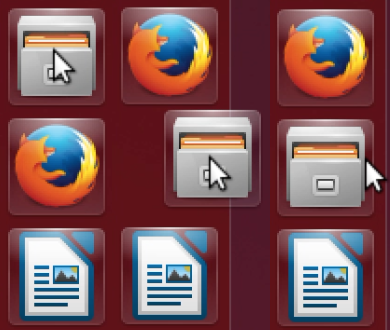
\includegraphics[width=\linewidth]{images/unity_launcher_zmiana_polozenia_ikon.png}
\end{wrapfigure}

Zawartość Launchera, poza ikoną Dasha oraz kosza, może być dowolnie modyfikowana. Aby zmienić położenie ikony na panelu, umieść kursor myszy nad ikoną, wciśnij i przytrzymaj lewy przycisk myszy. Kiedy ikona zostanie odczepiona od Launchera, przesuń ją na wybrane przez siebie miejsce i puść przycisk myszy.

\subsubsection{Dodawanie ikon do Launchera}
Skrót programu można dodać do Launchera na dwa sposoby. Pierwszy wykorzystuje okno Dasha (o którym będzie później). Aby dodać ikonę do paska bezpośrednio z Dasha, należy odszukać program i przeciągnąć jego ikonę w dowolne miejsce Launchera.

Druga metoda polega na uruchomieniu programu. Następnie należy kliknąć prawym przyciskiem myszy ikonę uruchomionego programu i z menu kontekstowego, które się pojawi, wybrać \textcolor{ubuntu_orange}{Dodaj do panelu uruchamiania}.

\subsubsection{Usuwanie ikon z Launchera}
Ikonę z paska można usunąć na dwa sposoby. Chwyć ikonę kursorem myszy i przenieś ją do kosza lub, po naciśnięciu ikony prawym przyciskiem myszy, z menu kontekstowego wybierz \textcolor{ubuntu_orange}{Usuń z panelu uruchamiania}.

\subsubsection{Szybka Lista menu kontekstowego (QuickList)}
\begin{center}
	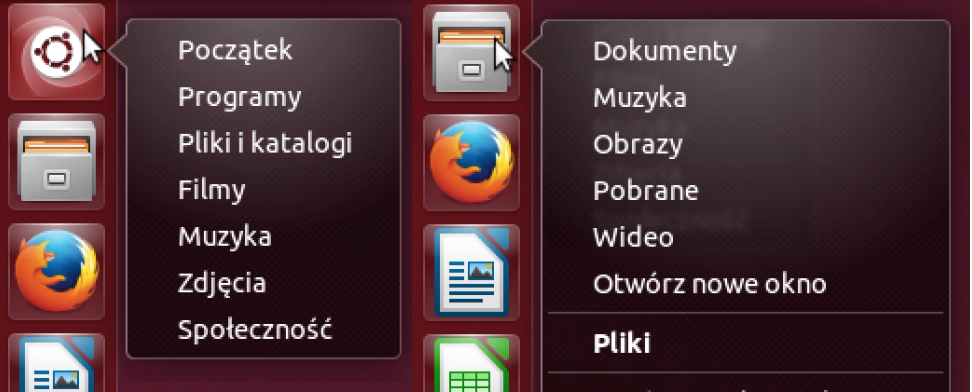
\includegraphics[width=\linewidth]{images/unity_launcher_quicklist.png}
\end{center}

QuickList (Szybka Lista) to jedna z ciekawszych funkcji Launchera. Po kliknięciu prawym przyciskiem myszy ikony programu w Launcherze pojawia się menu kontekstowe, w którym można umieścić różne polecenia. Na powyższej ilustracji widać dwa przykłady. Po lewej mamy menu kontekstowe Dasha, zawierające skróty do zainstalowanych soczewek (omówionych w kolejnym rozdziale). Po prawej widać menu kontekstowe menadżera plików, zawierające skróty do najważniejszych katalogów użytkownika. Przeglądarka internetowa Firefox pozwoli dodatkowo uruchomić okno anonimowego przeglądania.
\clearpage
